\documentclass[11pt]{article}
\usepackage[utf8]{inputenc}
\usepackage{geometry}
\usepackage{tikz}
\usetikzlibrary{arrows.meta}

% A fonte permanece a fonte padrão da classe article (Computer Modern).
\geometry{paperwidth=29.7cm,paperheight=13.6cm,margin=0cm}
\pagestyle{empty}

\definecolor{contorno}{RGB}{195,194,184}
\definecolor{cinzaTexto}{RGB}{83,83,83}
\definecolor{cinzaBarra}{RGB}{239,239,239}
\definecolor{azulContorno}{RGB}{39,115,215}
\definecolor{azulFundo}{RGB}{226,237,249}

\begin{document}
\noindent
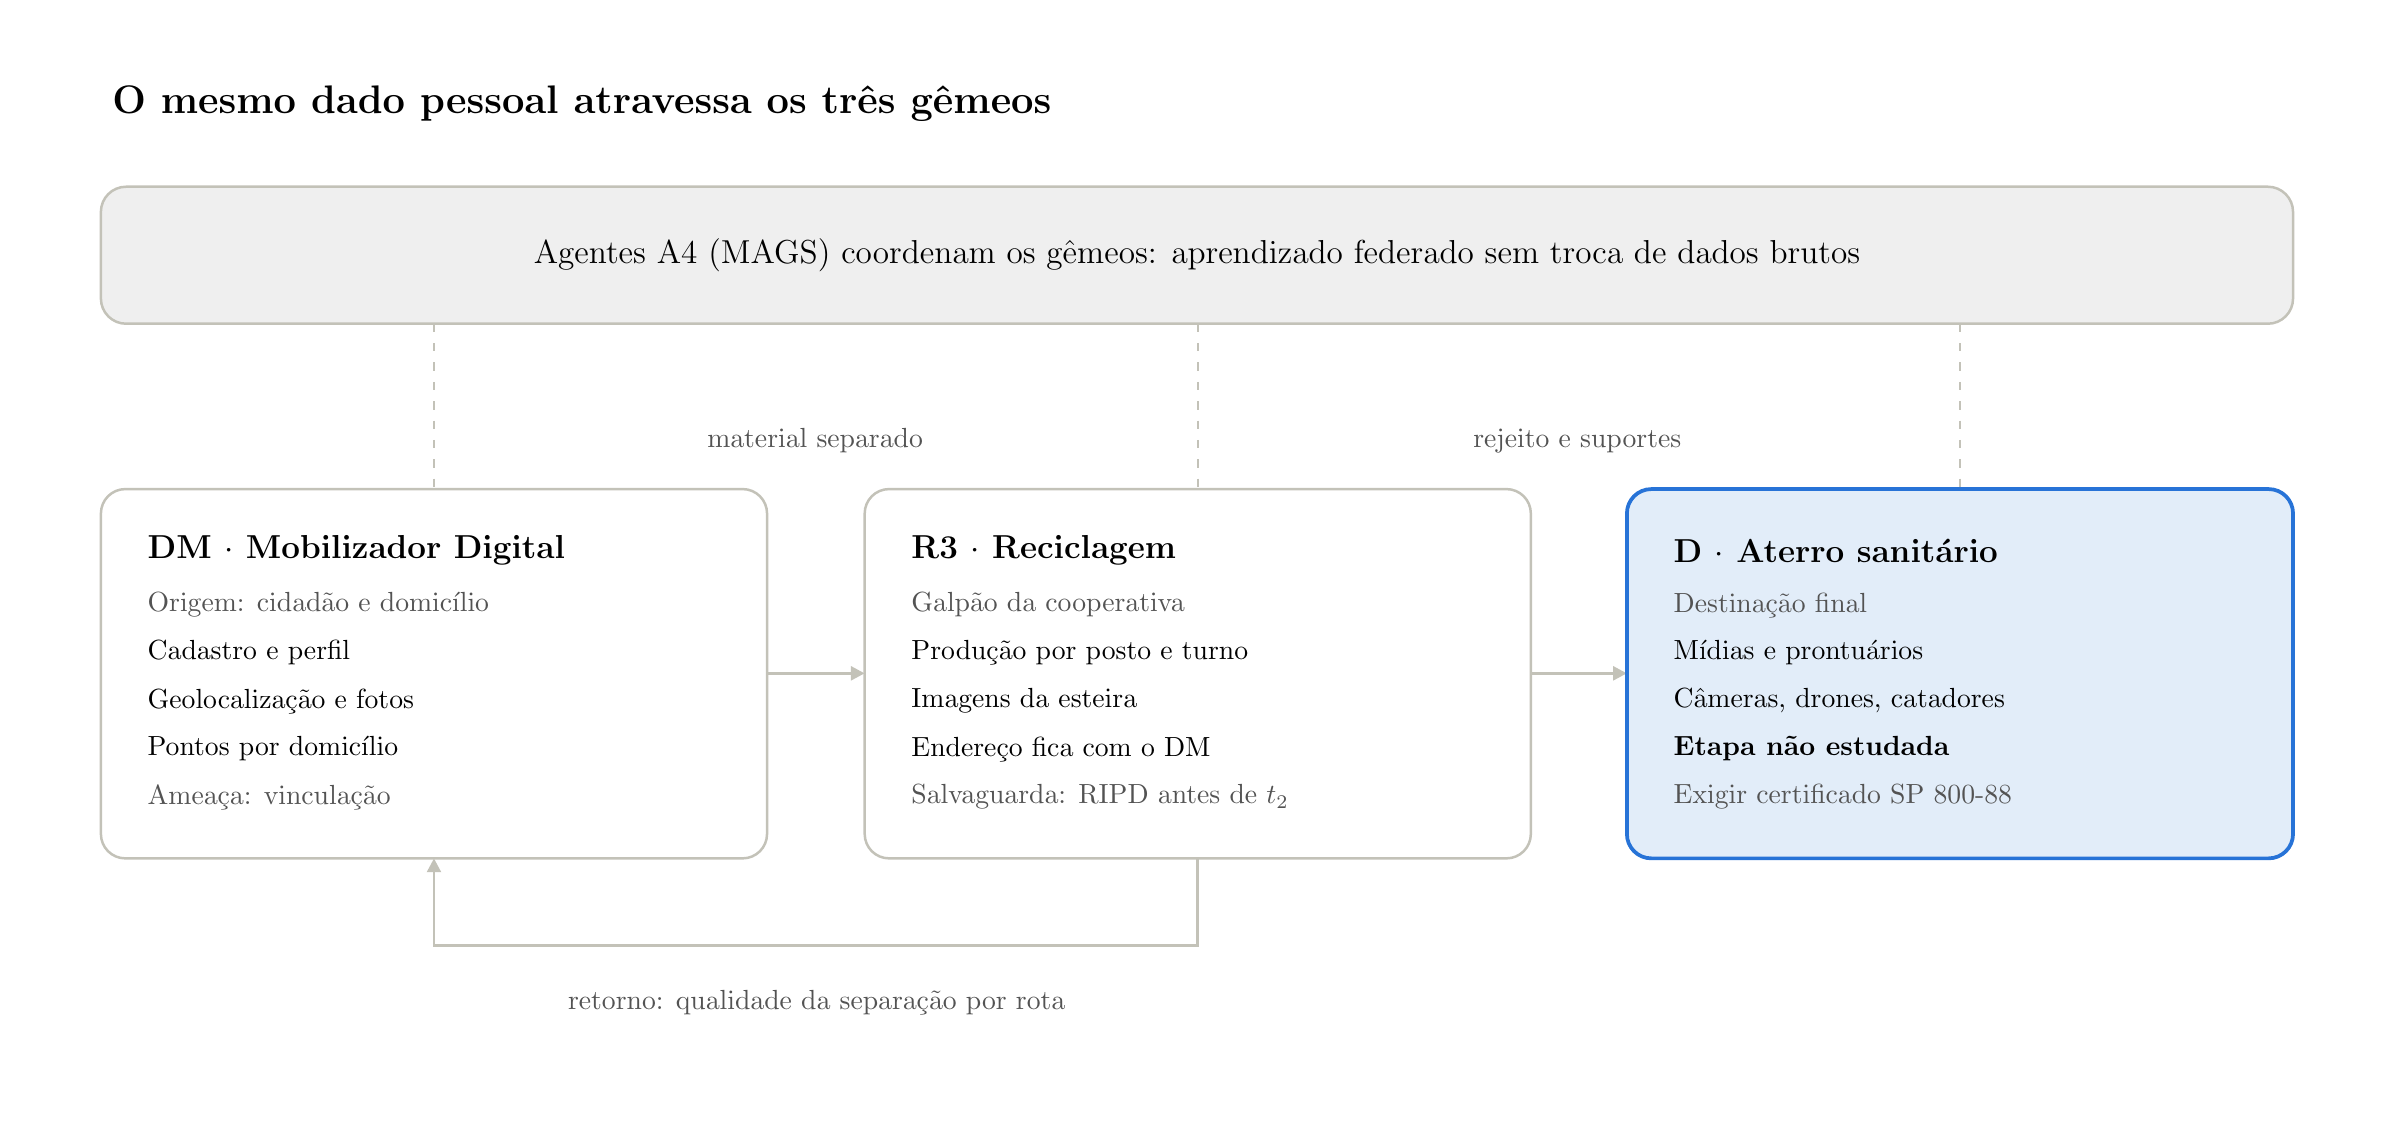
\begin{tikzpicture}[x=1cm,y=1cm]
  \path[use as bounding box] (0,0) rectangle (29.7,13.6);

  % Título e coordenação dos três gêmeos.
  \node[anchor=west,font=\bfseries\Large] at (0.95,12.64)
    {O mesmo dado pessoal atravessa os três gêmeos};
  \draw[fill=cinzaBarra,draw=contorno,line width=0.9pt,rounded corners=0.32cm]
    (0.93,9.84) rectangle (28.77,11.58);
  \node[font=\large] at (14.85,10.71)
    {Agentes A4 (MAGS) coordenam os gêmeos: aprendizado federado sem troca de dados brutos};

  % Ligações da coordenação com cada etapa.
  \foreach \x in {5.16,14.86,24.54} {
    \draw[draw=contorno,line width=0.75pt,dash pattern=on 3pt off 4pt]
      (\x,9.84) -- (\x,7.74);
  }

  % Fluxo principal e retorno de informação.
  \draw[draw=contorno,line width=1.1pt,-{Triangle[length=5pt,width=5pt]}]
    (9.39,5.40) -- (10.63,5.40);
  \draw[draw=contorno,line width=1.1pt,-{Triangle[length=5pt,width=5pt]}]
    (19.09,5.40) -- (20.31,5.40);
  \draw[draw=contorno,line width=1.0pt,-{Triangle[length=5pt,width=5pt]}]
    (14.86,3.05) -- (14.86,1.94) -- (5.16,1.94) -- (5.16,3.05);

  % Caixas das três etapas.
  \draw[draw=contorno,line width=0.9pt,rounded corners=0.31cm]
    (0.93,3.05) rectangle (9.39,7.74);
  \draw[draw=contorno,line width=0.9pt,rounded corners=0.31cm]
    (10.63,3.05) rectangle (19.09,7.74);
  \draw[fill=azulFundo,draw=azulContorno,line width=1.35pt,rounded corners=0.31cm]
    (20.31,3.05) rectangle (28.77,7.74);

  % Rótulos sobre as transições.
  \node[font=\normalsize,text=cinzaTexto] at (10.00,8.35) {material separado};
  \node[font=\normalsize,text=cinzaTexto] at (19.68,8.35) {rejeito e suportes};

  % DM — Mobilizador Digital.
  \node[anchor=west,font=\bfseries\large] at (1.40,6.96) {DM $\cdot$ Mobilizador Digital};
  \node[anchor=west,text=cinzaTexto] at (1.40,6.27) {Origem: cidadão e domicílio};
  \node[anchor=west] at (1.40,5.66) {Cadastro e perfil};
  \node[anchor=west] at (1.40,5.05) {Geolocalização e fotos};
  \node[anchor=west] at (1.40,4.44) {Pontos por domicílio};
  \node[anchor=west,text=cinzaTexto] at (1.40,3.83) {Ameaça: vinculação};

  % R3 — Reciclagem.
  \node[anchor=west,font=\bfseries\large] at (11.10,6.96) {R3 $\cdot$ Reciclagem};
  \node[anchor=west,text=cinzaTexto] at (11.10,6.27) {Galpão da cooperativa};
  \node[anchor=west] at (11.10,5.66) {Produção por posto e turno};
  \node[anchor=west] at (11.10,5.05) {Imagens da esteira};
  \node[anchor=west] at (11.10,4.44) {Endereço fica com o DM};
  \node[anchor=west,text=cinzaTexto] at (11.10,3.83)
    {Salvaguarda: RIPD antes de $t_2$};

  % D — Aterro sanitário.
  \node[anchor=west,font=\bfseries\large] at (20.78,6.96) {D $\cdot$ Aterro sanitário};
  \node[anchor=west,text=cinzaTexto] at (20.78,6.27) {Destinação final};
  \node[anchor=west] at (20.78,5.66) {Mídias e prontuários};
  \node[anchor=west] at (20.78,5.05) {Câmeras, drones, catadores};
  \node[anchor=west,font=\bfseries] at (20.78,4.44) {Etapa não estudada};
  \node[anchor=west,text=cinzaTexto] at (20.78,3.83)
    {Exigir certificado SP 800-88};

  \node[font=\normalsize,text=cinzaTexto] at (10.02,1.22)
    {retorno: qualidade da separação por rota};
\end{tikzpicture}
\end{document}
